% \documentclass{ijsra}
\def\IJSRAidentifier{\currfilebase} %<---- dont change this
\def\submission{}%YYYY-MM-DD
\def\acceptance{}%YYYY-MM-DD
%-------Title | Email | Keywords | Abstract-------------
\def\shorttitle{Classical Attic Grave Reliefs}
\def\maintitle{For \emph{Oikos} and \emph{Polis}:
	\\ Classical Attic Grave Reliefs as Family Monuments \\
	\emph{A Prosopographic Study of 14 Plaster Casts of Grave Reliefs from The Cast Gallery of the Ashmolean Museum, Oxford}}
\def\cmail{josephrobson96@yahoo.co.uk}
\def\keywords{Classical, Attica, Funerary Monuments, Public/Private Commemoration}
%\def\keywordname{}%<--- redefine the name \enquote*{Keywords}  in needed language
\def\abstract{Attic funerary stelai are a key source of material evidence for mapping changes within Attic self-perception and representation during the Classical period. A diverse range of family figures and social functions are depicted on stelai between their resurgence in c.430\BC and the reforms of Demetrios of Phaleron in c.317\BC. This article evaluates 14 plaster casts from the Cast gallery of the Ashmolean Museum in Oxford. The present corpus will be considered in an effort to evaluate the function of the monuments as commemorative markers, and how class and gender roles related to domestic and wider civil contexts. This article will evaluate any stylistic changes as they relate to potential changes within the conceptual family unit during this period, alongside the paradox of a private dedication erected in a public space. The purpose of this paper is to compile and scrutinise the many 20th and 21st century interpretations of Attic grave reliefs, in order to provide one’s own assessment on the intersectionality of stelai, the polis and the oikos. The paper serves as a contribution to recent scholarly attention on how the stele itself was an opportunity for familial promotion.}
%--------Author’s names------------
\def\authorone{Joseph Robson}
%-------Biographical information-------------
\def\bioone{Joseph Robson graduated from an Mst at the University of Oxford in 2018, having obtained his BA (Hons) in Classical Archaeology \& Ancient History from Oxford in 2017. Specialising in Numismatics and the history of collections, his Master's dissertation focuses on coin hoard patterns in late Iron Age and early Imperial Roman Britain (55\BC-\AD 93). He has volunteered at the Ashmolean Museum, Oxford, since 2014, in the galleries and Heberden Coin Room and interned at the British Museum’s coin department in 2017.}
%------University/Institution--------------
\def\affilone{Mst Classical Archaeology, University of Oxford}

\begin{filecontents}{\IJSRAidentifier.bib}
	%Bibliography-data HERE

	@book{Adam1966,
		author = {Adam, S.},
		title = {The Technique of Greek Sculpture in the Archaic and Classical Periods},
		date = {1966},
		publisher = {British School of Archaeology at Athens},
	}

	@article{Barker1924,
		author = {Barker, A.W.},
		title = {The Costume of the Servant on the Grave Relief of Hegeso},
		journaltitle = {American Journal of Archaeology},
		date = {1924},
		volume = {28},
		number = {3},
		pages = {290-292},
	}

	@book{Boardman1995,
		author = {Boardman, J.},
		title = {Greek Sculpture: The Late Classical Period},
		date = {1995},
		publisher = {Thames \& Hudson},
	}

	@incollection{Boegehold1994,
		author = {Boegehold, A.L.},
		title = {Perikles’s Citizenship Law of 451/50 BC},
		editor = {Boegehold, A.L. and Scafuro, A.C.},
		booktitle = {Athenian Identity and Civic Ideology},
		date = {1994},
		publisher = {John Hopkins University Press},
	}

	@article{Burton2003,
		author = {Burton, D.},
		title = {Public Memorials, Private Virtues: Women on Classical Athenian Grave Monuments},
		journaltitle = {Mortality},
		date = {2003},
		volume = {8},
		number = {1},
		pages = {20-35},
	}

	@book{Camp2001,
		author = {Camp, J.M.},
		title = {The Archaeology of Athens},
		date = {2001},
		publisher = {Yale University Press},
	}

	@book{Childs1998,
		author = {Childs, W.},
		title = {Reading Greek Art: Essays by Nikolaus Himmelmann},
		date = {1998},
		publisher = {Princeton University Press},
	}

	@book{Clairmont1995,
		author = {Clairmont, C.W.},
		title = {Classical Attic Tombstones: Introductory},
		date = {1995},
		publisher = {Kikhberg},
	}

	@article{Closterman2007,
		author = {Closterman, W.E.},
		title = {Family Ideology and Family History: The Function of Funerary Markers in Classical Attic Peribolos Tombs},
		journaltitle = {American Journal of Archaeology},
		date = {2007},
		volume = {111},
		number = {4},
		pages = {633-652},
	}

	@book{Frederiksen2011,
		author = {Frederiksen, R. and Smith, R.R.R.},
		title = {The Cast Gallery of Greek and Roman Sculpture: Catalogue of Plaster Casts of Greek and Roman Sculpture},
		date = {2011},
		publisher = {The Ashmolean Museum},
	}
	@article{Frel1973,
	author = {Frel, J.},
	title = {An Attic Grave Stele with Epigram},
	journaltitle = {Greek Roman and Byzantine Studies},
	date = {1973},
	volume = {14},
	number = {2},
	pages = {169-177},
}
	@book{Friis1951,
		author = {Friis Johansen, K.},
		title = {The Attic Grave Reliefs of the Classical Period: An Essay in Interpretation},
		date = {1951},
		publisher = {Ejnar Munksgaard},
	}

	@book{Fullerton2016,
		author = {Fullerton, M.D.},
		title = {Greek Sculpture},
		date = {2016},
		publisher = {Wiley Blackwell},
	}

		@book{Garland2001,
		author = {Garland, R.},
		title = {The Greek Way of Death},
		date = {2001},
		publisher = {Bristol Classical Press, London},
		Edition = {Second},
		pages = {21-106}
	}

	@incollection{Gray2011,
		author = {Gray, C.L.},
		title = {Foreigners in the Burial Ground: The Case of the Milesians in Athens},
		editor = {Carroll, M. and  Rempel, J. and Drinkwater, J.F. },
		booktitle = {Living Through the Dead: Burial and Commemoration in the Classical World},
		date = {2011},
		publisher = {Oxbow},
	}

	@book{Grossman2001,
		author = {Grossman, J.B.},
		title = {Greek Funerary Sculpture: Catalogue of the Collections at the Getty Villa},
		date = {2001},
		publisher = {Getty Publications},
	}

	@article{Grossman2007,
		author = {Grossman, J.B.},
		title = {Forever Young: An Investigation of the Depictions of Children on Classical Attic Funerary Monuments},
		journaltitle = {Hesperia Supplements},
		date = {2007},
		volume = {41},
		pages = {309-322},
	}

	@book{Hallett2005,
		author = {Hallett, C.H.},
		title = {The Roman Nude: Heroic Portrait Statuary 200 BC--AD 300},
		date = {2005},
		publisher = {Oxford University Press},
	}

	@book{Holwerda1899,
		author = {Holwerda, I.H.},
		title = {Die Attischen Gräber der Blüthezeit: Studien über die Attischen Grabreliefs},
		date = {1899},
		publisher = {Brill},
	}

	@book{Humphreys1993,
		author = {Humphreys, S.C.},
		title = {The Family, Women and Death: Comparative Studies},
		date = {1993},
		publisher = {University of Michigan Press},
	}

	@article{Hurwit2007,
		author = {Hurwit, J.M.},
		title = {The Problem with Dexileos: Heroic and Other Nudities in Greek Art},
		journaltitle = {American Journal of Archaeology},
		date = {2007},
		volume = {111},
		number = {1},
		pages = {35-60},
	}

	@book{Kurtz1971,
		author = {Kurtz, D.C. and Boardman, J.},
		title = {Greek Burial Customs},
		date = {1971},
		publisher = {Cornell University Press},
	}

	@article{Leader1997,
		author = {Leader, R.},
		title ={In Death Not Divided: Gender, Family and State on Classical Athenian Grave Stelae},
		journaltitle = {American Journal of Archaeology},
		date = {1997},
		volume = {101},
		pages = {683-699},
	}

	@book{Mee2011,
		author = {Mee, C.},
		title = {Greek Archaeology: A Thematic Approach},
		date = {2011},
		publisher = {Wiley-Blackwell},
	}

	@book{Neer2010,
		author = {Neer, R.},
		title = {The Emergence of the Classical Style in Greek Sculpture},
		date = {2010},
		publisher = {University of Chicago Press},
	}

	@incollection{Oliver2000,
		author = {Oliver, G.J.},
		title = {Athenian Funerary Monuments: Style, Grandeur and Cost},
		editor = {Oliver, G.J.},
		booktitle = {The Epigraphy of Death},
		date = {2000},
		pages = {59-80},
		publisher = {Liverpool University Press},
	}

	@book{Osborne1998,
		author = {Osborne, R.},
		title = {Archaic and Classical Greek Art},
		date = {1998},
		publisher = {Oxford University Press},
	}

	@book{Palagia2006,
		author = {Palagia, O.},
		title = {Greek Sculpture: Function, Materials, and Techniques in the Archaic and Classical Periods},
		date = {2006},
		publisher = {Cambridge University Press},
	}

	@article{Pemberton1989,
		author = {Pemberton, E.G.},
		title = {The Dexiosis on Attic Gravestones},
		journaltitle = {Mediterranean Archaeology},
		date = {1989},
		volume = {2},
		pages = {45-50},
	}

	@book{Pomeroy1997,
		author = {Pomeroy, S.},
		title = {Families is Classical and Hellenistic Greece: Representations and Realities},
		date = {1997},
		publisher = {Clarendon Press},
	}

	@article{Richter1954,
		author = {Richter, G.M.A},
		title = {Family Groups on Attic Grave Monuments},
		journaltitle = {Neue Beitrage zur Klassischen Altertumswissenschaft},
		date = {1954},
		volume = {60},
		pages = {256-262},
	}

	@book{Sourvinouinwood1995a,
		author = {Sourvinou-Inwood, C.},
		title = {Reading Greek Culture: Texts and Images, Rituals and Myths},
		date = {1995},
		publisher = {Clarendon Press},
	}

	@incollection{Sourvinouinwood1995b,
		author = {Sourvinou-Inwood, C.},
		title = {Male and Female, Public and Private, Ancient and Modern},
		editor = {Reeder, E.},
		booktitle = {Pandora: Women in Classical Greece},
		date = {1995},
		publisher = {Walters Art Gallery},
	}

	@book{Stamatopoulou1999,
		author = {Stamatopoulou, M.},
		title = {Burial Customs in Thessaly in the Classical and Hellenistic Periods},
		date = {1999},
		publisher = {DPhil Thesis},
	}

	@incollection{Stears1995,
		author = {Stears, K.},
		title = {Dead Women’s Society: Constructing Female Gender in Classical Athenian Funerary Sculpture},
		editor = {Spencer, N.},
		booktitle = {Time, Tradition and Society in Greek Archaeology: Bridging the \enquote*{Great Divide}},
		date = {1995},
		publisher = {Routledge},
	}

	@incollection{Stears2000a,
		author = {Stears, K.},
		title = {Losing the Picture: Change and Continuity in Athenian Grave Monuments in the Fourth and Third Centuries BC},
		editor = {Rutter, N.K. and Sparkes, B.A.},
		booktitle = {Word and Image in Ancient Greece},
		date = {2000},
		publisher = {Edinburgh University Press},
	}

	@incollection{Stears2000b,
		author = {Stears, K.},
		title = {The Times they are a changing: Developments in fifth-century Funerary Sculpture},
		editor = {Oliver, G.J.},
		booktitle = {The Epigraphy of Death: Studies in the History and Society of Greece and Rome},
		date = {2000},
		publisher = {Liverpool University Press},
	}

		@book{Stewart1990,
		author = {Stewart, A.},
		title = {Greek Sculpture: En Exploration},
		date = {1990},
		publisher = {Yale University Press},
		location = {New Haven},
		volume = {1-2},
		pages = {171-175}
	}

	@book{Strauss1993,
		author = {Strauss, B.S.},
		title = {Fathers and Songs in Athens: Ideology and Society in the era of the Peloponnesian War},
		date = {1993},
		publisher = {Princeton University Press},
	}

	@incollection{Stupperich1994,
		author = {Stupperich, R.},
		title = {The Iconography of Athenian State Burials in the Classical Period},
		editor = {Coulson, W.},
		booktitle = {The Archaeology of Athens and Attica under the Democracy},
		date = {1994},
		publisher = {Oxbow Monograph 37},
	}

	@article{Wasserman1969,
		author = {Wasserman, F.M},
		title = {Serenity and Repose: Life and Death on Attic Tombstones},
		journaltitle = {The Classical Journal},
		date = {1969},
		volume = {64},
		number = {5},
		pages = {193-202},
	}

	@book{Wrenhaven2012,
		author = {Wrenhaven, K.L.},
		title = {Reconstructing the Slave: The Image of the Slave in Ancient Greece},
		date = {2012},
		publisher = {Bristol Classical Press},
	}

	@book{Vonrodenwaldt1923,
		author = {Von Rodenwaldt, G.},
		title = {Das Relief Bei Dem Griechen},
		date = {1923},
		publisher = {Schoetz \& Parrhysius},
	}


\end{filecontents}
\IJSRAopening%<---- dont change this!
%-------
\lettrine{F}{unerary} \textit{stelai} of the Classical period are valuable material evidence for Athenian and Attic self-representation from c.430 \BC until the practice was banned by the tyrant Demterios in the reforms of c.317 \BC \parencite[100]{Pomeroy1997}.
The grave \textit{stele} was arguably a politicised medium for the depiction of the dead; its popularity correlates with the rise of less audacious grave goods, indicating a more modest alternative to the free-standing \textit{kouroi} and \textit{korai} of the \nth{6} century \BC \parencite[188]{Neer2010}.
A close analysis of the iconography of funerary stelai and accompanying inscriptions can often contribute to the identification of the deceased, relatives, attendants, careers and social standing of the subjects \parencite[20]{Burton2003}.
Greek grave reliefs have been extensively documented and researched since the late \nth{19} century. However, the breadth of research on Classical \textit{stelai} is not indicative of scholarly consensus. The diversity of the funerary iconographic palette has made identifying the subject of a grave relief a long-debated topic. The broad chronology of Classical \textit{stelai} is now widely considered to be orthodox, but the specific dating of an individual stele is rightly met by many with caution \parencite[16]{Clairmont1995}.
Stylistic assumptions can associate a \textit{stele} with a particular decade \parencite[113]{Adam1966}, but without accompanying inscriptions an exact date is not possible \parencite[5]{Grossman2001}.

Recently, Classical funerary sculpture has undergone a shift in scholarly focus. The last 15 years has seen greater interest in the evaluation of social history, especially the relationship between the domestic family unit (\textit{oikos}) and the wider political platform of the \textit{polis}. The purpose of this paper is to compile and scrutinise published works \nth{20} and \nth{21} century concerning Attic grave reliefs. There will be a particular focus on the relationship between the commissioning family’s intention for a \textit{stele}, and proceeding public reception. The intersectionality of stelai will be assessed, their iconography and context inexorably linked both to the \textit{polis} and the \textit{oikos}.

\IJSRAsection{\enquote*{Who is actually dead here?} An Immediate Complication}
Friis Johansen’s landmark text on classical grave reliefs sought to resolve an ongoing problem in interpretation \parencite[53]{Friis1951}.
Namely, the issue of identifying which figure or figures were the deceased on a pair or group scene. A controversial study by Holwerda in 1899 argued that grave reliefs did not depict the deceased, and has since been dismissed \parencite{Holwerda1899}.
Mynno’s stele (\ref{fig:Robson_Figure_01}) bears only an inscribed name and a solitary, seated young woman.
There is no evidence to suggest the figure was a relative or grave attendant and not Mynno herself. The research consensus agrees instead that solo mortal figures must be the deceased \parencite[119]{Stears1995}.
Attic reliefs of pairs are similarly straightforward. Hegeso (\ref{fig:Robson_Figure_03}) and Dexileos (\ref{fig:Robson_Figure_12}) are named and feature in pairs.
The standing figure on stele \ref{fig:Robson_Figure_03} wears a hair-net and double-chiton, holding a pyxis for the seated woman to inspect \parencite[292]{Barker1924}.
The former is subservient, an ancillary figure whose presence visualises the aristocratic status of Hegeso \parencite[689]{Leader1997}.
The nude male on stele \ref{fig:Robson_Figure_12} is pierced by a spear but few Attic grave reliefs depict the moment of a subject’s death; the figure is Dexileos’ defeated foe \parencite[57]{Hurwit2007}.
Both examples illustrate how secondary characters are easily identifiable by their costume and relation to the central figure \parencite[53]{Friis1951}.
Although Fullerton suggests that the Dexileos stele would have been a \enquote*{stock composition}, the visual and emotional impact of a heroic death in combat is not diminished \parencite[549]{Fullerton2016}.

Identifying the deceased within a family group is a more complex task. Friis Johansen maintains that the homogeneity of the genre’s iconography is the cause of confusion \parencite[55]{Friis1951}.
For example, grave reliefs did not depict portraiture, unlike some free-standing statues in the mid-\nth{4} century. The subjects of funerary reliefs are idealised versions, crafted to be symbolic and not precise representations of figures \parencite[313]{Grossman2007}.
Furthermore, the approaches utilised on solo or pair scenes are not necessarily applicable to group scenes \parencite[62]{Vonrodenwaldt1923}.
For example, \textit{stele} \ref{fig:Robson_Figure_06} shows an elderly bearded man on a chair, demonstrating that the funerary image of the seated figure was not exclusive to women. On \textit{stele} \ref{fig:Robson_Figure_09} the seated woman is on the far right of the relief, secondary to the elevated reclining male. The image of a seated woman is repeated alongside other visual cues that would have otherwise identified them as the deceased.

\IJSRAsection{ \enquote*{Life} after Death.  A Cause for Commemoration}

Despite ongoing and detailed scholarly research, identifying the exact context of a scene presents a challenge that has not yet been resolved. Defining the scene beyond an interior or exterior setting often risks being contradictory or impenetrable at worst \parencite[53]{Friis1951}.
One controversial aspect of this debate comes with attempting to explain the significance of family scenes \parencite[26]{Stears2000a}.
The previous section outlines how the deceased is not only represented on grave \textit{stelai}, but is the main subject of the scene. In single figure scenes like \textit{stele} \ref{fig:Robson_Figure_01} or \ref{fig:Robson_Figure_13} identification is highly convincing.
Apart from monuments like \ref{fig:Robson_Figure_08} and \ref{fig:Robson_Figure_14} which contain \enquote*{competing}™ iconography, it is usually possible to ascertain who the deceased is and who is a relative/child/slave in the scene \parencite[175]{Frel1973}.

Since the late \nth{19} century three major theories approach the confusion of scenes with multiple family members. Firstly, the deceased is intended to occupy the realm of the dead, with the surrounding family as survivors brought together by grief \parencite[116]{Boardman1995},
or perhaps the deceased is bidding farewell to the living before starting his or her spiritual journey into the afterlife \parencite[116]{Boardman1995}.
Secondly, the scene takes place entirely in the afterlife with a grand reunion \parencite[247]{Mee2011}.
Third, the \textit{stele} acts as a bridge between the realms of the living and the dead \parencite[198]{Wasserman1969}. One social theme transcends the different hypotheses and is found in all four: the oikos was the essential concept for understanding the Attic family unit, and had to be nurtured and accepted by the polis.

The idea of a dead figure surrounded by surviving family members has been championed by Kurtz and Boardman \parencite[140]{Kurtz1971},
and is consistent with this report’s view that family members funded the production of the actual relief \parencite[96]{Wrenhaven2012}.
The most compelling evidence for this theory comes from stele 11, Excavated from the Ilissos River. The nude subject of the scene leans against the anta, as an elderly male figure stands passively to his right. His gaze is locked on the face of the deceased, leaning gently against his staff and raising his right hand to his chin in contemplation \parencite[141]{Kurtz1971}.
The old man’s quiet intensity seeks to connect to the heroic male, who is oblivious to his presence as he stares out into the world of the viewer. Nevertheless, the elder remains an important ancillary figure in the intergenerational scene '€“ He is draped in a thick himation, a civic garment that alludes to active participation in the public affairs of the polis \parencite[20]{Hallett2005}.
The dichotomy between the pair ultimately defines the elder as a bystander to the youth, who exudes a passive, detached presence \parencite[145]{Palagia2006}.

A similar distinction appears in \textit{stele} \ref{fig:Robson_Figure_10}, where Telesias observes a hare without returning the gaze of the child beside him. Kurtz and Boardman consider this separation to visually divide life and death in Attic funerary iconography.
Family or servants on monuments like \textit{stele} \ref{fig:Robson_Figure_03} are spectators to the deceased subject, just like the actual visitor to the grave (Wrenhaven, 2012:101).
The clasping of hands (dexiosis) appears in \textit{stelai} \ref{fig:Robson_Figure_04}, \ref{fig:Robson_Figure_06}\ref{fig:Robson_Figure_08}, \ref{fig:Robson_Figure_14}, and possibly denotes the \enquote*{final farewell}™ and retirement of the subject from the realm of the living \parencite[247]{Mee2011}.

By combining dexiosis and the physical disconnect between figures, \textit{stelai} reflect the perpetuity of the oikos in Athenian and Attic society \parencite[23]{Pomeroy1997},
death was inherently disruptive to the operation of the oikos \parencite[128]{Stears1995}.
Indeed, the majority of the report’s \textit{stelai} depict those who died \enquote*{prematurely}: mothers with infants, hoplites, cavalrymen and unmarried girls \parencite[119]{Stears1995}.
A survey of Attic gravestones reveals 34 cases of a father who left behind a child or children \parencite[111]{Humphreys1993}.
By commissioning a \textit{stele} depicting the dead alongside living family members, the dedicator conveys two important messages. They recognise that the oikos had been threatened by an untimely death, but it is strong enough to survive the family tragedy. The oikos was a major expression of Attic identity in the Classical period \parencite[3]{Grossman2001}.
As a result, the death of a young citizen like Dexileos in \textit{stele} \ref{fig:Robson_Figure_12} would have threatened the family unit’s property inheritance and family legacy \parencite[62]{Gray2011}.

On balance, the theory of surviving family observing the deceased is a possible explanation for family scenes on grave reliefs. The absence of an important figure in the oikos could be publicly recognised through signs of either tenderness or a lack thereof. Furthermore, the presence of relatives in funerary scenes represents the survival of the family unit despite the death. In death an individual departed from the household and the oikos, but the oikos as an Attic ideology lived on \parencite[23]{Pomeroy1997}.

Conversely, Pemberton argues that the farewell theory is incidental, and applied retroactively by modern scholarship \parencite[50]{Pemberton1989}.
Indeed, the imagery of deceased/survivor scenes is not seen in all grave reliefs. \textit{Stelai} \ref{fig:Robson_Figure_01} and \ref{fig:Robson_Figure_13} are solitary scenes so there is no interaction with other figures.
In addition, \textit{stelai} \ref{fig:Robson_Figure_02} and \ref{fig:Robson_Figure_09} are damaged, missing heads or basic facial details.
Therefore signs of familial fondness are hard to identify. The indifference of the Ilissos stele youth was unlikely to have been a motive of the sculptor \parencite[14]{Clairmont1995}. \nth{4} century \BC funerary sculpture broadly followed to the sculptural style first seen on the Parthenon frieze \parencite[197]{Osborne1998}.
As such Classical grave reliefs followed the trend of more serene compositions \parencite[195]{Wasserman1969}.
However, these traits do not explain the expressions of the \enquote*{surviving}™ figures. Some basic level \textit{stelai} were not personalised except for an inscription, which further challenges the farewell theory \parencite[66]{Oliver2000}.

Humphreys suggests an alternative: that group scenes on Attic gravestones show a complete family reunion in the afterlife \parencite[106]{Humphreys1993}. \textit{Stele} \ref{fig:Robson_Figure_07} is this catalogue’s sole example which explicitly corroborates this view.
Depicting two women inscribed as Demetria and Pamphile, \textit{stele} \ref{fig:Robson_Figure_07} was excavated from the burial plot of the same two women from the Kerameikos \parencite[256]{Richter1954}.
Recent scholarship largely agrees that \textit{stele} \ref{fig:Robson_Figure_07} was the second monument erected on the plot and was constructed after the death of Pamphile \parencite[636]{Closterman2007}.
The original stele commemorating Demetria remained on the same burial plot as the amended \textit{stele}, so didn'€™t serve a purely pragmatic purpose. Humphreys proposes that scenes of family reunion are a visual illustration of family-owned burial plots \parencite[2]{Humphreys1993}.
Burying family members alongside one another in plots that were terraced and walled from the rest of the Kerameikos emphasised familial affection \parencite[114]{Boardman1995}.
The case of Demetria and Pamphile is evidence for the elite of Athens, but is not directly representative of aristocratic ideals in the wider Attic region. A scene cut as deep as the relief of \textit{stele} \ref{fig:Robson_Figure_07} in a family plot was a luxury only attainable by the wealthiest families \parencite[124]{Sourvinouinwood1995b}.
The depth of many \nth{4} century \BC \textit{stelai} also allows for more artistic compositions and greater variety in busier group scenes \parencite[185]{Neer2010}.
Many peribolos and family tombs at Athenian and Attic cemeteries do not follow suit, implying that similar scenes were not a reunion in the afterlife but an ageless and idealised depiction of the deceased as in life \parencite[194]{Wasserman1969}. The reunion theory is less compelling than the \enquote*{farewell}™ theory, because the supporting evidence is extremely rare.

\IJSRAsection{The Significance of Dexiosis}

The third theory about Attic perceptions of the afterlife forges a middle ground between the theories of farewells or reunions. The handshake (\textit{dexiosis}) often appears in funerary iconography, and boasts a rich Greek cultural history \parencite[96]{Stupperich1994}.
\textit{Dexiosis} appears on Attic grave monuments from the \nth{5} century \BC resurgence onwards, the clasping of hands symbolising accord between two parties of equal standing, publicly reaching a position of mutual agreement over a decision \parencite[49]{Pemberton1989}.

The handshake holds a spiritual significance in burial rites, as a symbol linking the living and the deceased in Attic society \parencite[115]{Boardman1995}.
From a stylistic perspective \textit{dexiosis} demonstrates how the surviving family recognised the private and public roles of deceased during their life, and wished to publicly display their achievements \parencite[321]{Grossman2007}.
Curiously the gesture is largely absent from the archaeological pottery record \parencite[138]{Kurtz1971}, except for white-ground lekythoi from the late \nth{5} century \BC that could be mistaken for passing a physical object to another. The modern historian can retroactively apply a range of social/gender-based connotations to the \textit{dexiosis} image.

Overall, the iconography of Attic grave monuments is difficult to decipher without reference to contemporary and earlier Greek art. The idea of a reunion scene is only relevant to a minority of grave reliefs, and the evidence is circumstantial. Boardman’s theory of survivors (simultaneously complementing the deceased’s position within the polis while alive and their journey into the afterlife) is also problematic \parencite[116]{Boardman1995}.
It is an effective illustration of an honourable burial being the reward for being an active member of one’s oikos \parencite[193]{Wasserman1969}. Grave reliefs were the perfect means of communicating such sentiments to the wider polis, with wealthy families competing to erect the grandest monument.

\IJSRAsection{Happy Home, Happy Polis}

Funerary monuments in Attic grave precincts celebrate the contribution of a man or woman to the \textit{oikos}. Presenting their domestic role in a funerary space within a \textit{polis} was an opportunity to convey private achievements to a wider audience \parencite[3]{Grossman2001}.
However, considering the public sphere as a vehicle for solely private commemoration fails to accept that the oikos and polis as social institutions were inextricably linked \parencite[17]{Pomeroy1997}.
In the early \nth{21} century prosopography has seen a much needed rise in scholarly interest \parencite[172]{Stamatopoulou1999}, wherein grave \textit{stelai} are re-evaluated as evidence for socio-political processes of Attic poleis, and a common burial custom \parencite[25]{Stears2000b}.
Notably, of this article’s reliefs that depict exclusive family scenes only four show a harmonious family unit through the previously discussed \textit{dexiosis} motif. The image of an idealised oikos is deliberately used to mirror the prosperity of the polis \parencite[699]{Leader1997}.
Grave reliefs of mothers hold a particular social significance, potentially as a response to the Periklean citizenship legislation of 451/0 \BC \parencite[648]{Closterman2007}.
The explicit depiction of one’s lineage added a legal dimension to grave \textit{stelai}, subtly promoting the theme of \textit{anchisteia} in a public space (Stears, 1995:114).

In the case of \textit{stele} \ref{fig:Robson_Figure_06}, dated tentatively to c.360 \BC, an elderly man rests on a chair, clasping hands with a young woman while a youth watches.
The gesture displays multiple generations of the same family, publicly depicted as virtuous sharing the same family ideology \parencite[651]{Closterman2007}.
Close contact is also shown by the youth who rests his right palm gently upon the elder’s right shoulder, so all three characters are physically connected. Both standing figures are visibly younger than \textit{Arkesilas}, but because Attic women were married in their teenage years mere observation is insufficient in distinguishing whether the woman in \textit{stele} \ref{fig:Robson_Figure_06} (\ref{fig:Robson_Figure_07}) was his wife or daughter \parencite[26]{Clairmont1995}.
Despite this drawback, \textit{stele} \ref{fig:Robson_Figure_06} remains an effective example of how the ideology of the family was a factor in the decoration of a funerary monument, arguably more so than proclaiming one’s property \parencite[193]{Osborne1998}.
Even though \textit{stele} \ref{fig:Robson_Figure_06} lacks an explicit reference to using lineage as a means of securing citizenship, it hints at how the medium could be utilised in such a way \parencite[648]{Closterman2007}.

Grave monuments did not explicitly document the legal status of their subjects \parencite[651]{Closterman2007}.
Rather, the higher number of mortal women depicted in relief than in other monumental art forms is an intriguing comparison. It implies that grave reliefs were an ideological proclamation of citizenship to the polis of the deceased. One explanation is the Periklean citizenship law of c.450 \BC.
The legislation decreed that a mother had to be the daughter of an Athenian citizen for her son to be a legal Athenian citizen, in an attempt to reduce the size of the citizen body (Plutarch Perikles 37.3). As a result, proving one’s birth to an Athenian mother was necessary to secure citizenship (Isaeus On the Estate of Philoctemon 6.64), and the lineage had to be confirmed across at least two generations \parencite[24]{Burton2003}.
Citizenship laws also correlate to the commission of family scenes that depict children or grandchildren of the deceased \parencite[25]{Burton2003}.

The iconography of \textit{stele} \ref{fig:Robson_Figure_08} encapsulates a stele’s aspirational function of closely associating with the polis \parencite[126]{Pomeroy1997}.
In particular, a nude infant reaches for his mother, who is shaking hands with a bearded man clad in full military regalia. The servant girl, carrying a \textit{pyxis} akin to \textit{stelai} \ref{fig:Robson_Figure_02} and \ref{fig:Robson_Figure_03}, exists as a symbol of the family’s aristocratic status.
The foot soldier’s helmet and cuirass were only worn by the hoplite class, closely associating the male figure with the state. Finally, the woman and baby explicitly express the child’s participation in both a private and public setting, a suitable candidate for citizenship by Perikles’ regulations established in the previous century \parencite[312]{Grossman2007}.
Overall, the rise of grave monuments portraying family groups inherently forms a stylistic change which features a greater prominence of women. The imagery of multiple generations alongside a seated or standing mother presents the family unit as a social institution with legal importance. If the mother is the subject the immediate family is implicitly portrayed as seeking legal security, more so than a social statement on women in society \parencite[60]{Boegehold1994}.

Following the re-emergence of decorated gravestones from the 430’s \BC, there was a different approach to their spatial organisation in the funerary space. Namely, the rising popularity of family plots by the end of the \nth{5} century could be a direct response to the social legislature of the Athenian \textit{polis}. Whether the response was positive or negative has been the subject of strong scholarly debate. By c.425 \BC approximately 10\% of all Athenian families owned a family plot, including \textit{stelai} \ref{fig:Robson_Figure_03}, \ref{fig:Robson_Figure_07}, and \ref{fig:Robson_Figure_12} \parencite[41]{Stears2000b}.
Crucially this doesn’t mean that family members were buried together; only three out of 598 published graves between the \nth{6} and \nth{4} centuries \BC contained relatives buried next to each other \parencite[124]{Pomeroy1997}.
The Hegeso and Dexileos reliefs still suggest that the trend persisted for decades after it first appeared, because both were erected in the 390’s \BC (IG ii 6226-30).
The relief of Demetria and Pamphile is from c.320 \BC and shares a similar context. However, using a single, later relief is too selective an approach to confirm the widespread trend of family grave plots throughout the \nth{4} century \BC.

The imagery of family scenes and inscriptions exudes \textit{aréte} A state of moral virtue and fulfilment, either as an individual or an entire family \parencite[117]{Sourvinouinwood1995b}.
Plato lauds this virtue, stating that a successful Greek longed for wealth and honour among peers. A citizen should \enquote*{bury one’s parents well} and receive the same treatment from their own children (Plato Hippias Major 291).
Plato confirms the centrality of commemorative burial rites in Attic society \parencite[22]{Garland2001}, and implies that agathe among Attic men was a universal virtue, expected in both the polis and the oikos settings. Grave reliefs were therefore microcosms for the complementary nature of the public and private spheres.
A citizen’s duty varied, but the principles of modesty and honour were essential \parencite[32]{Burton2003}.
Such virtues were created and exchanged by both spheres. For this reason the decoration of a grave relief sought to praise the deceased and their family as members of their oikos, because it promulgated their virtue as citizens of their polis \parencite[41]{Strauss1993}.

The reliefs of Hegeso, Dexileos, and Demetria and Pamphile are exceptionally decorated reliefs, and among the largest in size of the report catalogue. The higher cost of deeper and more elaborate reliefs indicates that the trend may have seen greater prominence among elite Athenian families \parencite[54]{Sourvinouinwood1995b}.
Nearby Attic sites like Menidi and Chalandri are less comprehensively published, making it difficult to compare the cases from Athens to their Attic contemporaries.
Individual finds like \textit{stele} \ref{fig:Robson_Figure_11} (Found in the Ilissos river in 1874) are less compatible with a broader line of investigation \parencite[218]{Frederiksen2011}.
Sourvinou-Inwood reinforces the idea of subtle aristocratic changes occurring gradually in Classical grave reliefs, but this is not necessarily representative of other Attic cities or poleis \parencite[416]{Sourvinouinwood1995a}.

On the contrary, \textit{stelai} \ref{fig:Robson_Figure_09} and \ref{fig:Robson_Figure_10} from the early-to-mid \nth{4} century \BC Piraeus
\enquote{displaying a banquet scene and a possible hunt scene respectively}
 account for the range and complexity of funerary iconography.
Both scenes may record the deceased’s preference for feasts or hunting while he was still alive, or contain subtle religious connotations \parencite[187]{Stamatopoulou1999}.
In the case of \textit{stele} \ref{fig:Robson_Figure_09}, the reclining man immediately draws a parallel to the symposium \parencite[186]{Stamatopoulou1999}.
His languid posture and attendant to the left of the scene reveal a higher social status, achievable by his nobility and personal wealth. Such examples remind the historian that grave monuments formed part of a commercial market with differing social and religious significance for each client \parencite[175]{Stewart1990}.
There are broad stylistic or ritual trends like the rise in family burial plots \parencite[164]{Camp2001}. Sculptors and buyers did not have to conform to contemporary trends, and as such earlier motifs continued alongside innovative designs.

\IJSRAsection{Career as the Height of Life. Military and Athletic Depictions of Men}

The deceased are depicted on gravestones either in the afterlife or as if they were still alive \parencite[115]{Boardman1995}.
Women are usually shown performing household tasks or inspecting personal jewellery on grave reliefs (\ref{fig:Robson_Figure_01}, \ref{fig:Robson_Figure_02}, \ref{fig:Robson_Figure_03}, \ref{fig:Robson_Figure_05} and \ref{fig:Robson_Figure_08});
their role within the oikos \parencite[20]{Burton2003}.
The reliefs show them at their most beautiful, wealthy or dutiful to their family \parencite[117]{Sourvinouinwood1995b}.
On the other hand male figures were depicted at the peak of their civic careers for Athens or the wider Attic region. Men are shown participating in athletics, warfare, trade or politics  all taking place in the public eye \parencite[21]{Burton2003}.
Such roles allowed the state to function, and helped to achieve and consolidate the security and prosperity of the state \parencite[27]{Burton2003}.
Fullerton maintains that the grave stele was a primarily personal rather than political monument \parencite[542]{Fullerton2016}. However, the overt imagery of costumes or nudity shows that political or public motivations are also a significant factor.

In 404/3 \BC Athens lost the Peloponnesian War against the Lacedaemonians. An almost 30 year old conflict ended with a year of Athens being ruled by the 30 tyrants, before restoring the democratic system of government (Xenophon Hellenica 2.4.1). The final quarter of the \nth{5} century \BC had seen the destruction of Attic farmland by Spartan troops in the 420’s \BC (Thucydides 2.18-23), the failure of the Piraeus as a supreme naval hub for the Athenian empire, and conflicts against Corinth in 394/3 \BC which are noted on \textit{stele} \ref{fig:Robson_Figure_12}. Grave reliefs \enquote{unlike state burials} were an opportunity to recognise the contribution of an individual to his city. Funerary stelai could show that Attic society perceived the idealised citizen to be a man willing to die for the protection of his \textit{polis}.

One explanation for nude male figures on grave reliefs is that they were athletes, or hunters in some scenes. \textit{Stele} \ref{fig:Robson_Figure_10} is an example of the latter, and displays Telesias in the nude resting his weight onto one hip.
Nudity in sculpture was not an invention of the Classical period, the majority of Greek archaic \textit{kouroi} were naked, drawing the viewer’s eye to the subject’s defined musculature as the ideal image for an athletic youth \parencite[115]{Boardman1995}.
Hallett posits that nudity would have been the \enquote*{uniform} of the gymnasium, the term itself deriving from gymnos (naked) \parencite[22]{Hallett2005}.
The suggested formal approach renders the image of the nude beardless youth both idealised and widely recognisable to the contemporary Attic viewer. The same can be said for \textit{stele} \ref{fig:Robson_Figure_11}, where the deceased is imagined in peak physical fitness and an idealised representation that was attainable by male athletes and soldiers \parencite[94]{Stupperich1994}.
The fine details of the naked body on \textit{stele} \ref{fig:Robson_Figure_11} allowed for a more nuanced pose: frozen on the cusp of movement, twisting his torso to his right \parencite[200]{Osborne1998}.

The style is reminiscent of variations of the Polykleitan walking motif, creating the impression of vitality that has been captured or cut short before reaching their maximum potential \parencite[163]{Childs1998}.
Such a trait has featured on earlier stelai including the marker of Chairodemos and Lykeas \parencite[162]{Childs1998}.
Youthful energy and a strong physique exaggerate the subject’s physical prowess, but can also highlight the tragic circumstances of the subject’s departure. Grave monuments dedicated to youths were paid for by their father or wider family, and publicly express sorrow at this subversion of the natural order, as described by Plato \parencite[195]{Wasserman1969}. \textit{Stele} \ref{fig:Robson_Figure_11} evokes grief through its explicit dichotomy between figures;
the heavily-draped elder contrasts the youth’s nude image \parencite[116]{Boardman1995}.
The relief on \ref{fig:Robson_Figure_12} is an exception because Dexileos is fully armoured while his victim in naked. For the most part the sculpting of naked men had the effect of heroising their mortal involvement in the polis.

The stele of Demokleides (\ref{fig:Robson_Figure_13}) from the Piraeus deserves further evaluation as a depiction of military service, due to its naval iconography. A rower sits beside his armour on the prow of his ship, the details of which are tantalisingly fragmentary.
Crucially, the Demokleides stele is the only known Attic grave monument from the Classical period to feature a rower or a naval vessel. Out of the hundreds of excavated grave monuments, images of the hoplites and cavalrymen were far more common \parencite[97]{Stupperich1994}.
This comparison is evident in both state burials and private dedications \parencite[97]{Stupperich1994}. Thucydides maintains that rowers were historically the driving force behind the Athenian empire in the early \nth{5} century \BC, implying a shift during the classical period. Indeed, the scarcity of grave reliefs depicting rowers may be a sign of a declining reliance on the navy, in the eyes of the polis (Thucydides 1.93).

In funerary sculpture, the rarity of naval imagery could hold a social significance in addition to its explicitly martial message. Dexileos’s inscription (\ref{fig:Robson_Figure_12}) commemorates the valour of the shock cavalry at Athens.
Dexileos’s elite role against Corinth was worthy of special mention, among the \enquote*{five riders} on the frontline. On the other hand, Demokleides’s inscription states that he was lost at sea in c.394 \BC \parencite[197]{Wasserman1969}.
It mourns his tragic loss instead of singling out his actions as a heroic Athenian warrior. When considered in conjunction with the iconography and subjects of state burials in Athens and Attica, the conclusion is twofold. Firstly, hoplites seem to be prioritised by the Attic polis through state commissioned grave monuments. Secondly, the families of hoplites and cavalrymen were of a higher class than the families of rowers, hence the more elaborate and plentiful reliefs on record \parencite[97]{Stupperich1994}. Despite some minor iconographic differences, it is clear that military and athletic participation was idealised in funerary relief sculpture. For Athenian and Attic men, their public careers were the most important contribution to the \textit{polis}, and was capitalised upon in death.

\IJSRAsection{Concluding Remarks}

Attic grave reliefs of the Classical period are valuable social documents, but are not without significant drawbacks. They contribute to our comprehension of the role of the individual and the family, acting paradoxically as private memorials on public display. Unfortunately, it is often a complicated and problematic process to identify the deceased in each scene. This greatly limits our understanding of the intentions and beliefs of the individuals who commissioned a funerary monument. Contemporary and later literature from Thucydides, Diodorus Siculus and Plutarch help to contextualise some of the social themes conveyed on grave reliefs, such as the desire to enforce male hegemony and the spiritual importance of family unity and \textit{dexiosis}. The grave monument heroised the dead as a praiseworthy citizen who ranked his duty to the polis above all else. The rarity of naval scenes could also highlight a shift from Athens as a naval power (since its defeat in 404 \BC) to a greater focus on its land armies.

There are inherent problems when dating individual grave reliefs, because any attempts are set against a chronology which is based almost entirely on relative dates. With the exception of inscriptions recording the archon years of the subject’s death (namely \textit{stele} \ref{fig:Robson_Figure_12}), a stylistic interpretation can only pinpoint broad trends in the classical style. As a result it would be ill-advised to assign a particular relief to a specific event, unless it was known to have had a lasting effect on the Attic region. For example, the citizenship laws of 451/0 \BC arguably inspired the newfound prominence of Athenian women and the position of the mother in the family after the re-emergence of grave reliefs, in an attempt to secure the family estate. The 317 \BC funerary legislation of Demetrios abruptly ended the decorative bombast of later grave monuments. The law acknowledged how competition among the social elite was originally curbed in the late \nth{6} or early \nth{5} century \BC, but had returned to Attic funerary practices in the 430’s \BC. The concept had firmly ingrained itself in later grave reliefs, which partly explains the popularity of funerary monuments as a medium for self-promotion. Dedicators accentuated the deceased’s career in the polis, either publicly or implicitly through the running of the oikos. When considered in tandem with the sometimes blatant attempts to maximise visibility in grave precincts, the public praise they sought to generate would contribute to the family manifesto.

The oikos cannot be ignored on funerary scenes, because prosperity in the individual household was considered a crucial underlying factor in the long-term success of the polis. Indeed, the ultimate focus of attic grave reliefs was directed firmly towards the polis. The legacy of the deceased individual, the benefits of a family dedicated relief, and the consolidation of social status are all achieved through Attic grave monuments.


\IJSRAseparator
\clearpage
\IJSRAsection{CATALOGUE}

See all figures after Reference Section.

\begin{figure}[!b]
	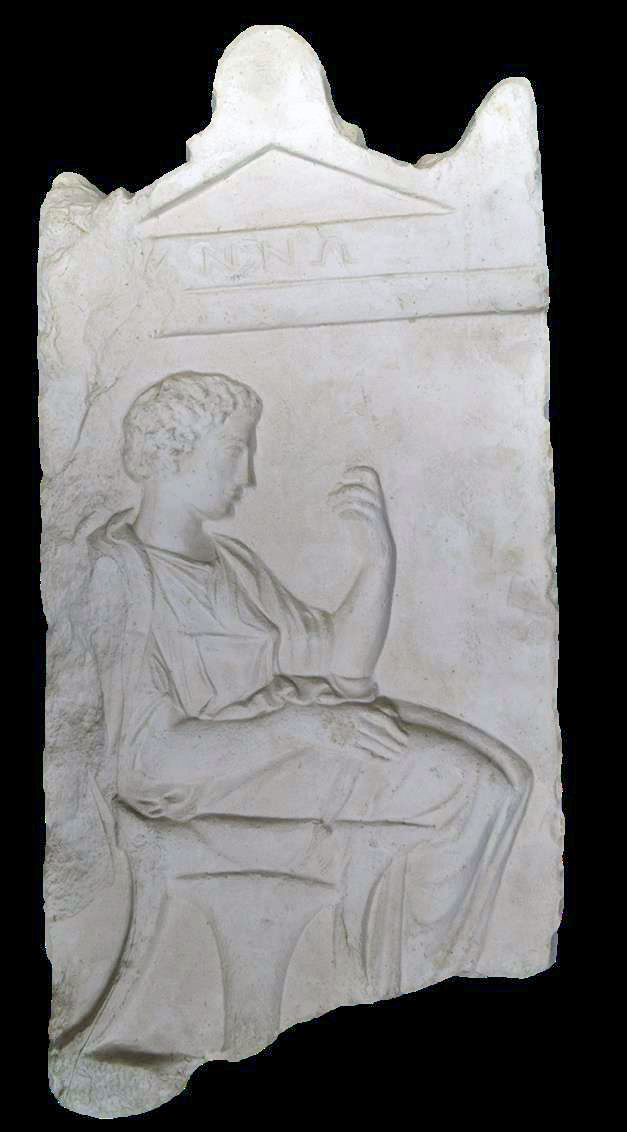
\includegraphics[width=0.7\linewidth]{Robson_Figure_01}

	\caption{Grave stele of Mynno. Oxford, Ashmolean Cast Gallery Inv. D039; Berlin, Antikensammlung, Staatliche Museen zu Berlin Inv. 737; Late 5 century \BC, Pentelic Marble; Attica, between Athens and the Piraeus; Height: 60cm, Width: 28cm; Bibliography: TCG, 207, D039; CAT 2, 1.176; DAG 1, 38.17. Comparanda: D037
		{\normalfont\scriptsize \\ \copyright\ by Joseph Robson}}
	\label{fig:Robson_Figure_01}
\end{figure}
\clearpage
\begin{figure}[!p]
	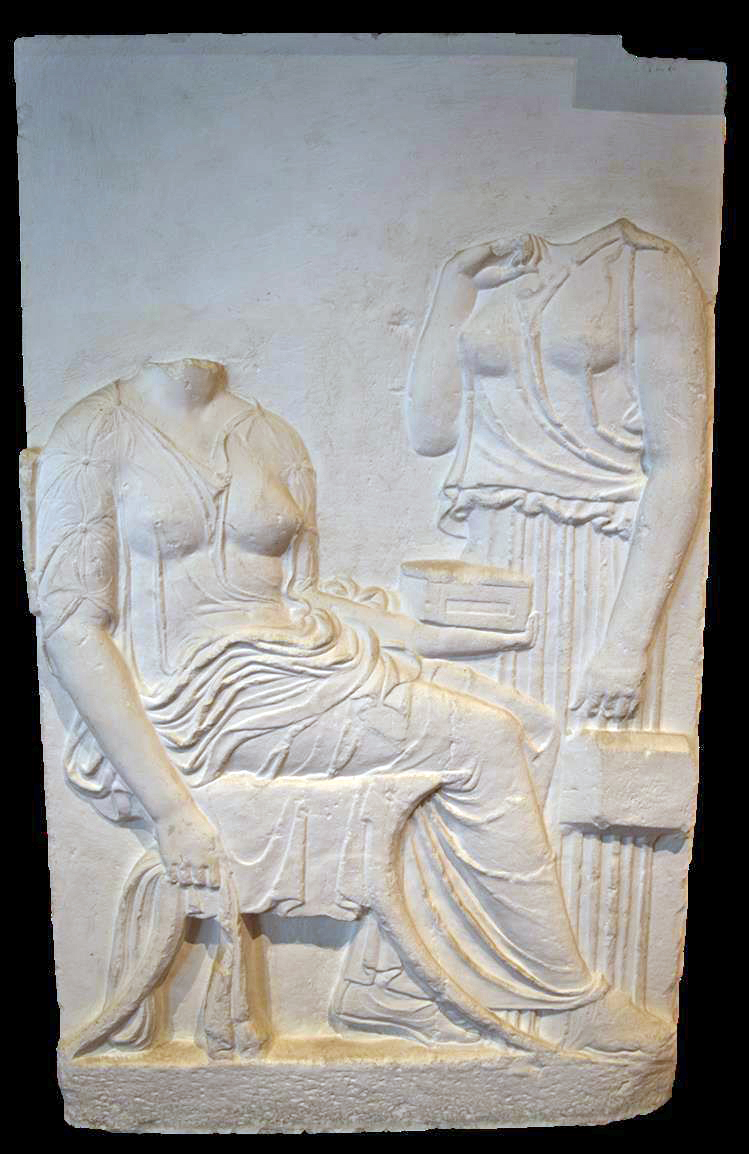
\includegraphics[width=.8\linewidth]{Robson_Figure_02}

	\caption{Grave stele of seated woman. Oxford, Ashmolean Cast Gallery Inv. D038; Athens, National Archaeological Museum Inv. 1822; Late 5th century \BC, Marble; Athens, between Athinas Street \& Lykourgou Street (lower part found in 1898, upper part found in 1964)
		Height: 1.18m, Width: 70cm; Bibliography: TCG, 207, D038; CAT 2, 98, 2.151.
		Comparanda: D037; NAM, inv. 820; inv. 831.
		{\normalfont\scriptsize \\ \copyright\ by Joseph Robson}}
	\label{fig:Robson_Figure_02}
\end{figure}
\clearpage
\begin{figure}[!p]
	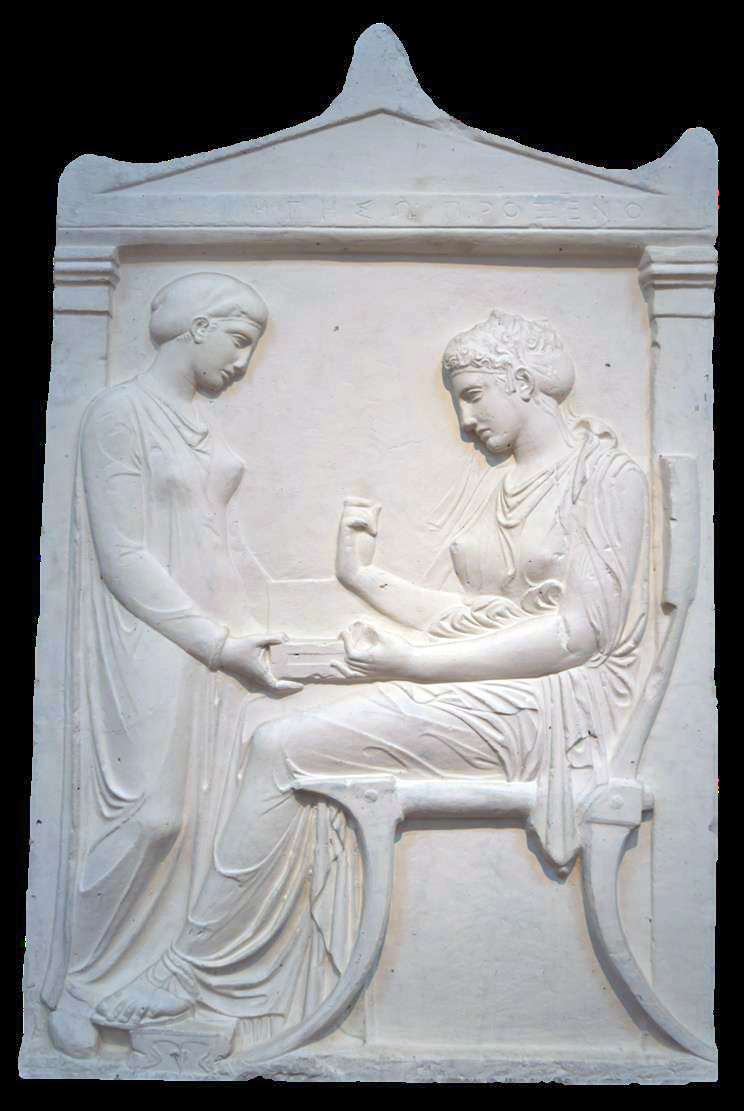
\includegraphics[width=\linewidth]{Robson_Figure_03}

	\caption{Grave stele of Hegeso. Oxford, Ashmolean Cast Gallery Inv. D037. Athens, National Archaeological Museum Inv. 3624; c.400 \BC, Pentelic Marble; Athenian Kerameikos (Discovered in 1870); Height: 1.5m, Width: 97cm; Bibliography: TCG, 207, D037; CAT 2, 95-9, 2.150; DAG 1, 21, 68. Comparanda: D038; D039; NAM, inv. 1178a; inv. 726.
		{\normalfont\scriptsize \\ \copyright\ by Joseph Robson}}
	\label{fig:Robson_Figure_03}
\end{figure}
\clearpage
\begin{figure}[!p]
	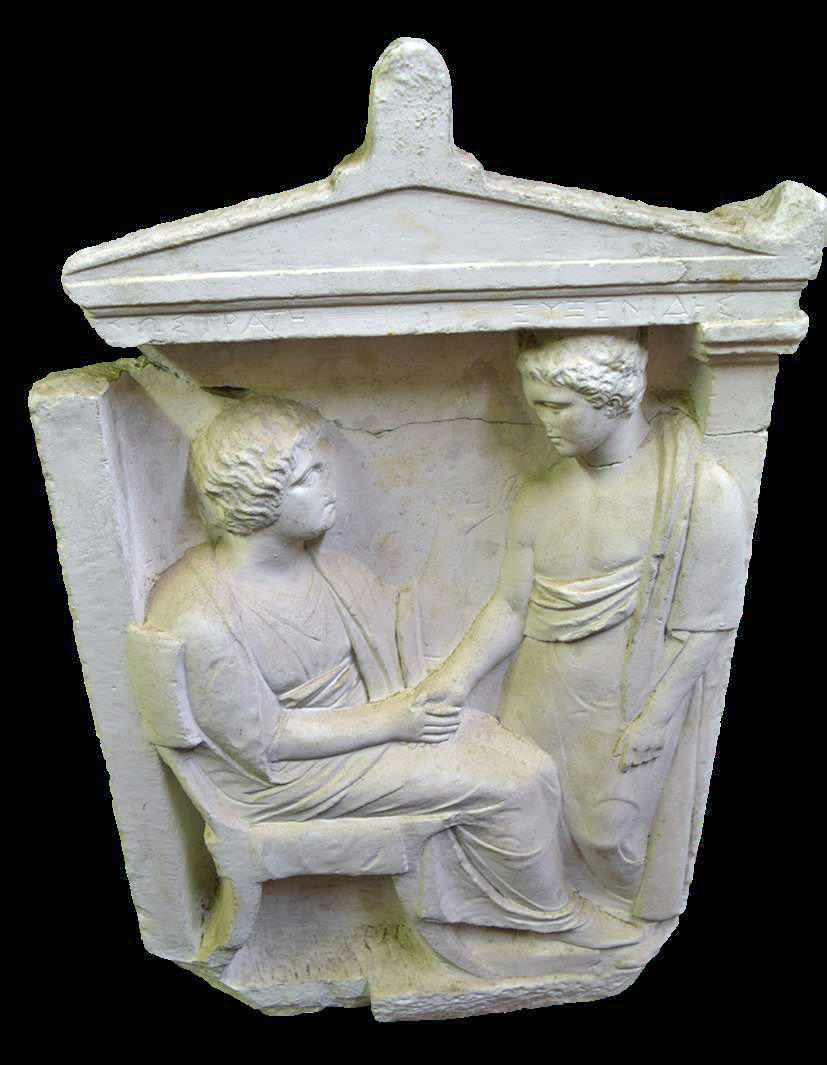
\includegraphics[width=\linewidth]{Robson_Figure_04}

	\caption{Grave stele of Sostrate and Euxenides. Oxford, Ashmolean Cast Gallery Inv. D072; Copenhagen, Ny Carlsberg Glyptothek Inv. 1695; Early 4th century \BC, possibly Pentelic Marble; Menidi, Attica; Height: 1.03m, Width: 60 cm; Bibliography: TCG, 217, D072; CAT 2, 206, 2.227b. Comparanda: NAM, inv. 765.
		{\normalfont\scriptsize \\ \copyright\ by Joseph Robson}}
	\label{fig:Robson_Figure_04}
\end{figure}
\clearpage
\begin{figure}[!p]
	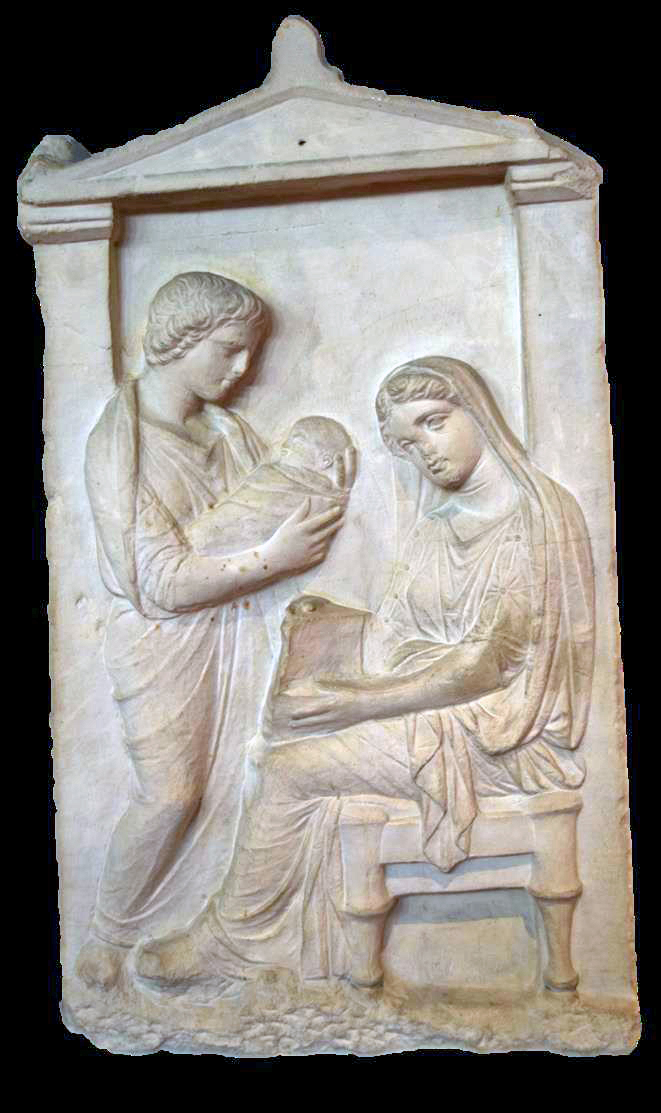
\includegraphics[width=.8\linewidth]{Robson_Figure_05}

	\caption{Grave stele of a mother. Oxford, Ashmolean Cast Gallery Inv. D073; London, British Museum Cat. 2232; Early 4th century \BC, Pentelic Marble
		Attica; Height: 80cm, Width: 46cm; Bibliography: TCG, 217, D073; CAT 2, 691, 2.786. Comparanda: NAM, inv. 722; inv. 3790.
		{\normalfont\scriptsize \\ \copyright\ by Joseph Robson}}
	\label{fig:Robson_Figure_05}
\end{figure}
\clearpage
\begin{figure}[!p]
	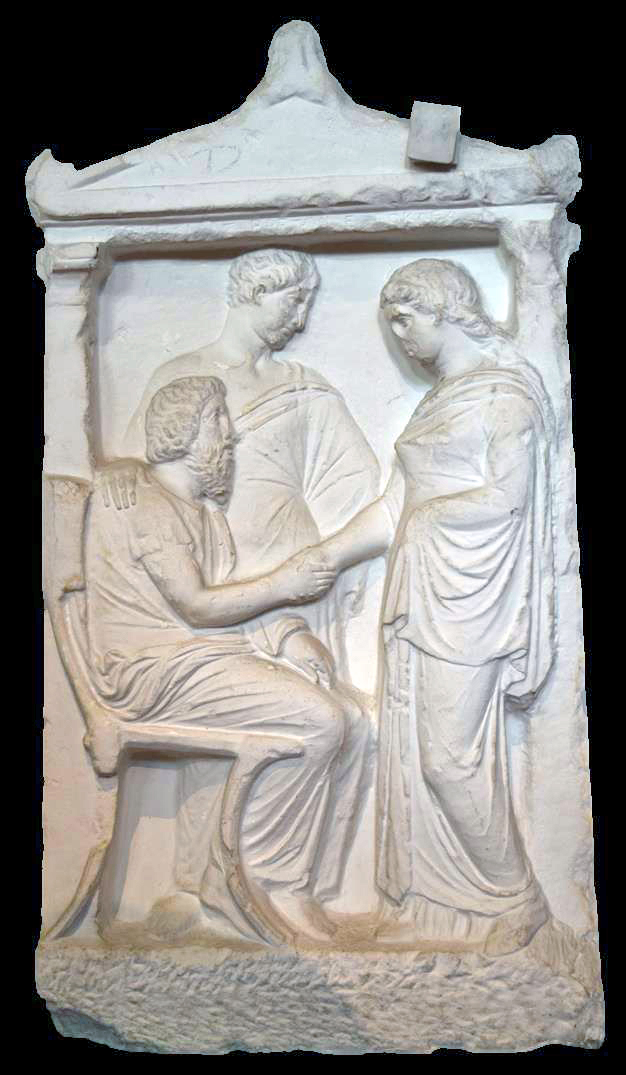
\includegraphics[width=.8\linewidth]{Robson_Figure_06}

	\caption{Grave stele of Arkesilas. Oxford, Ashmolean Cast Gallery Inv. D075; Dresden, Albertinum Inv. ZV 2440 (Hm 144); c. 360 \BC, Pentelic Marble; Athens; Height: 89cm, Width: 49cm; Bibliography: TCG, 218, D075; CAT 3, 242-4, 3.374c. Comparanda: NAM, inv. 902.
		{\normalfont\scriptsize \\ \copyright\ by Joseph Robson}}
	\label{fig:Robson_Figure_06}
\end{figure}

\clearpage
\begin{figure}[!p]
	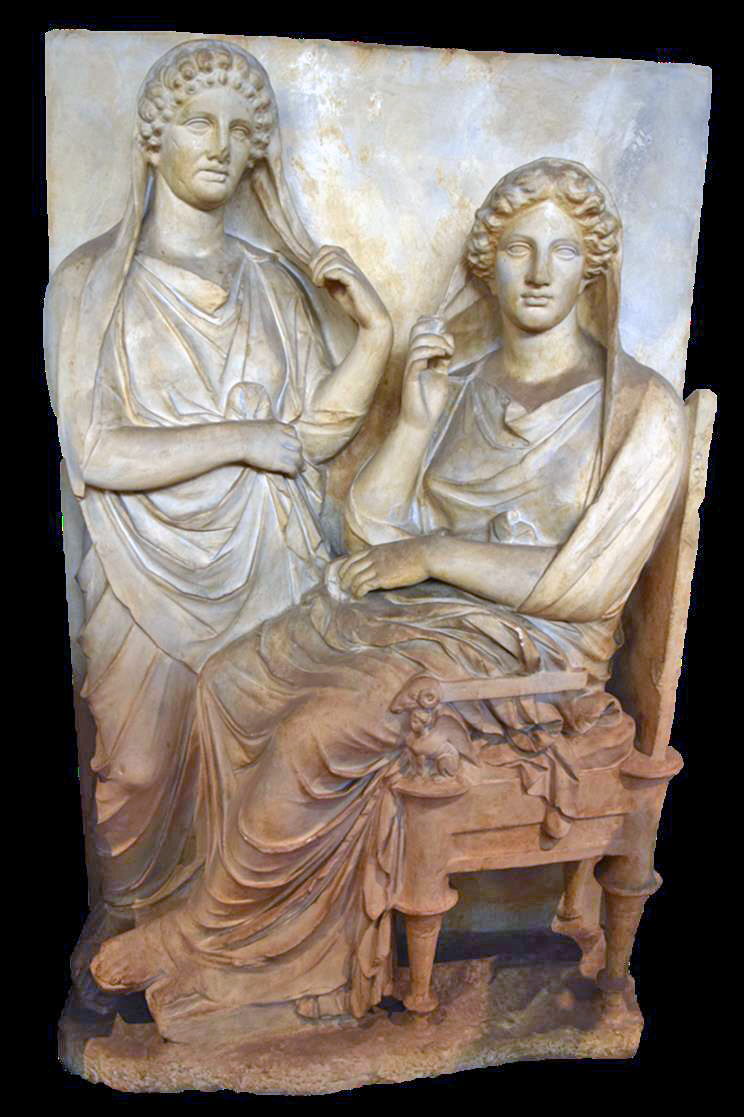
\includegraphics[width=.9\linewidth]{Robson_Figure_07}

	\caption{Grave stele of Pamphile; Oxford, Ashmolean Cast Gallery Inv. D077; Athens, Kerameikos Museum; C. 320 \BC, Pentelic Marble; Athenian Kerameikos (Found in 1870); Height: 1.98m, Width: 1.25m; Bibliography: TCG, 218, D077; CAT 2, 593-5, 2.464; DAG 1, 30-1, 109.40. Comparanda: NAM, inv. 724; inv. 819; inv. 743; inv. 820.
		c
		{\normalfont\scriptsize \\ \copyright\ by Joseph Robson}}
	\label{fig:Robson_Figure_07}
\end{figure}
\clearpage

\begin{figure}[!p]
	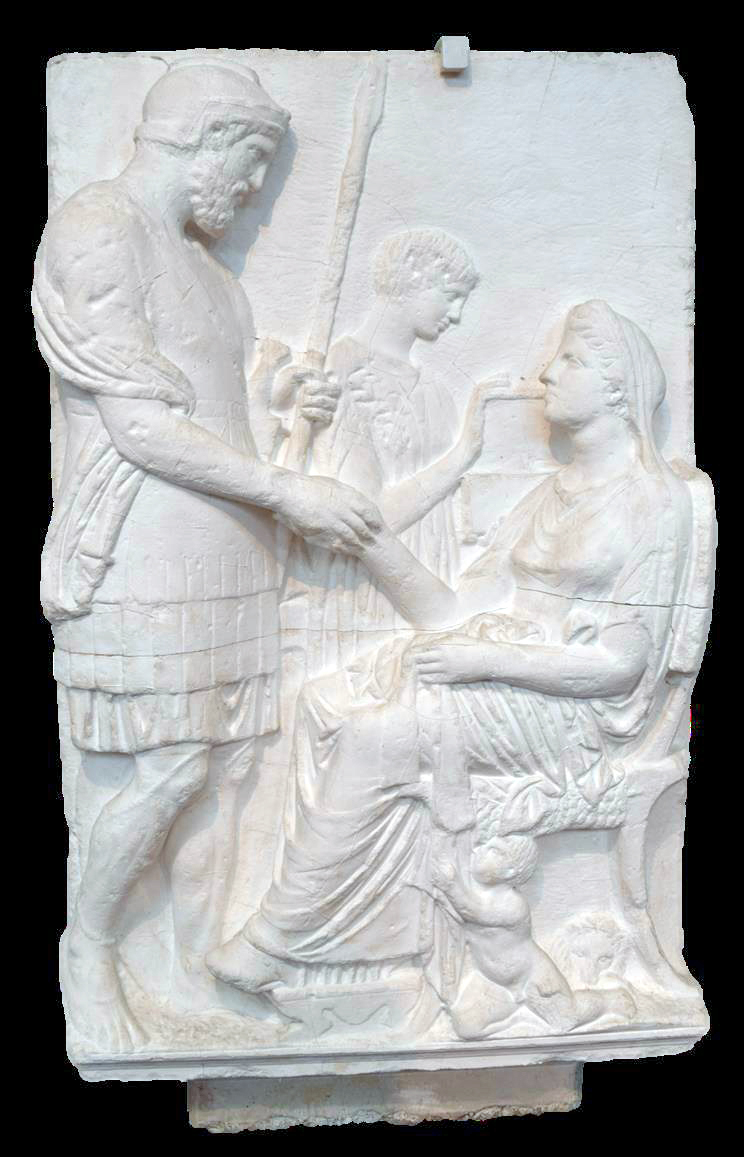
\includegraphics[width=.9\linewidth]{Robson_Figure_08}

	\caption{Grave stele of hoplite and family. Oxford, Ashmolean Cast Gallery Inv. D069; Berlin, Antikensammlung Staatliche Museen zu Berlin Inv. 1473. Attica; C. 350 \BC, Pentelic Marble; Height: 1.76m, Width: 1.1m. Bibliography: TCG, 216, D069; DAG 1, 107, 463.
		Comparanda: D065; NAM, inv. 834
		{\normalfont\scriptsize \\ \copyright\ by Joseph Robson}}
	\label{fig:Robson_Figure_08}
\end{figure}
\clearpage
\begin{figure}[!p]
	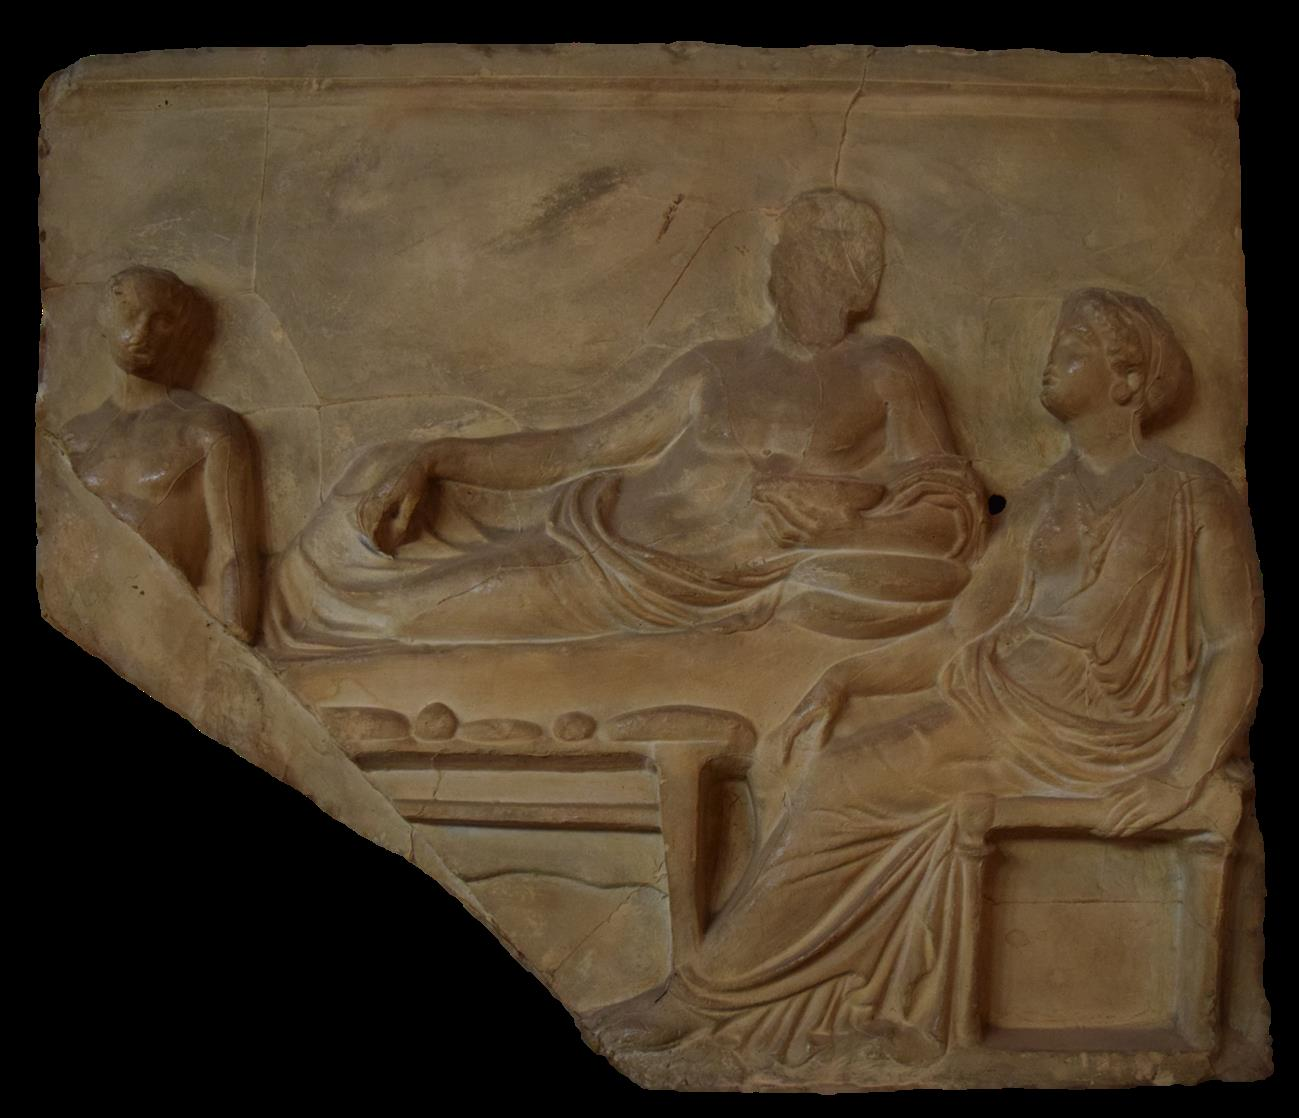
\includegraphics[width=\linewidth]{Robson_Figure_09}

	\caption{Grave stele of a reclining male. Oxford, Ashmolean Cast Gallery Inv. D082; Piraeus, Archaeological Museum Inv. 208; c. 380\BC, Marble; Piraeus, Athens; Height: 57\,cm, Width: 64\,cm; Bibliography: TCG, 220, D082.
		{\normalfont\scriptsize \\ \copyright\ by Joseph Robson}}
	\label{fig:Robson_Figure_09}
\end{figure}
\clearpage
\begin{figure}[!p]
	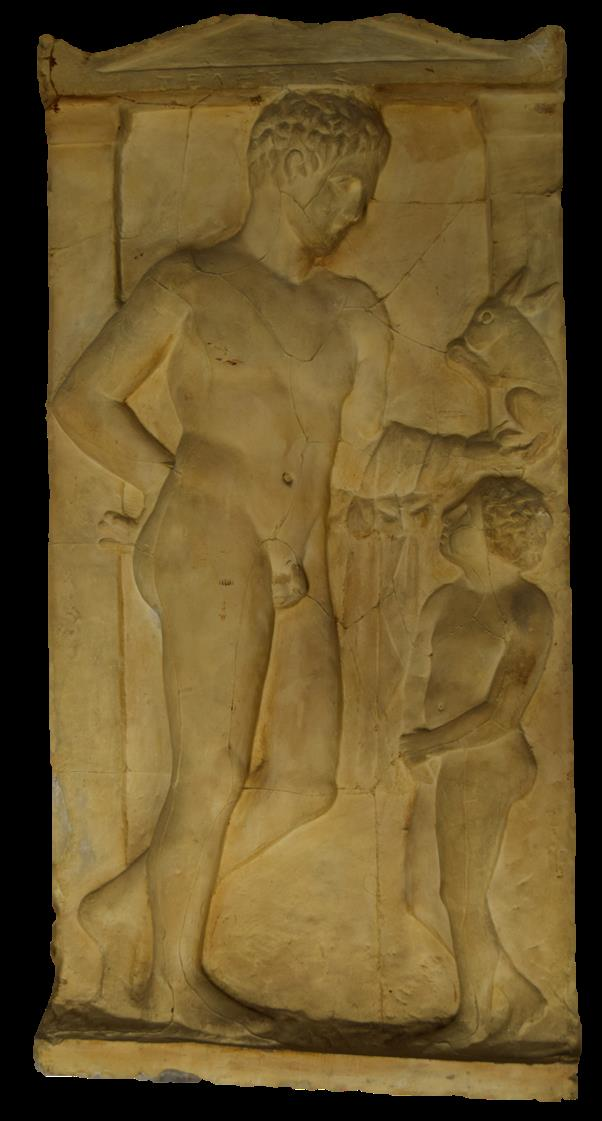
\includegraphics[width=.7\linewidth]{Robson_Figure_10}

	\caption{Grave stele of Telesias. Oxford, Ashmolean Cast Gallery Inv. D071; Athens, National Archaeological Museum Inv. 898. 370-360 \BC, Marble. Piraeus (Found in 1871); Height: 77cm, Width: 40cm; Bibliography: TCG, 217, D071; CAT 1, 448-9, 1.810; DAG 2, 221-2, 1036.208.
		Comparanda: NAM, inv. 715; inv. 914; inv. 794.
		{\normalfont\scriptsize \\ \copyright\ by Joseph Robson}}
	\label{fig:Robson_Figure_10}
\end{figure}
\clearpage
\begin{figure}[!p]
	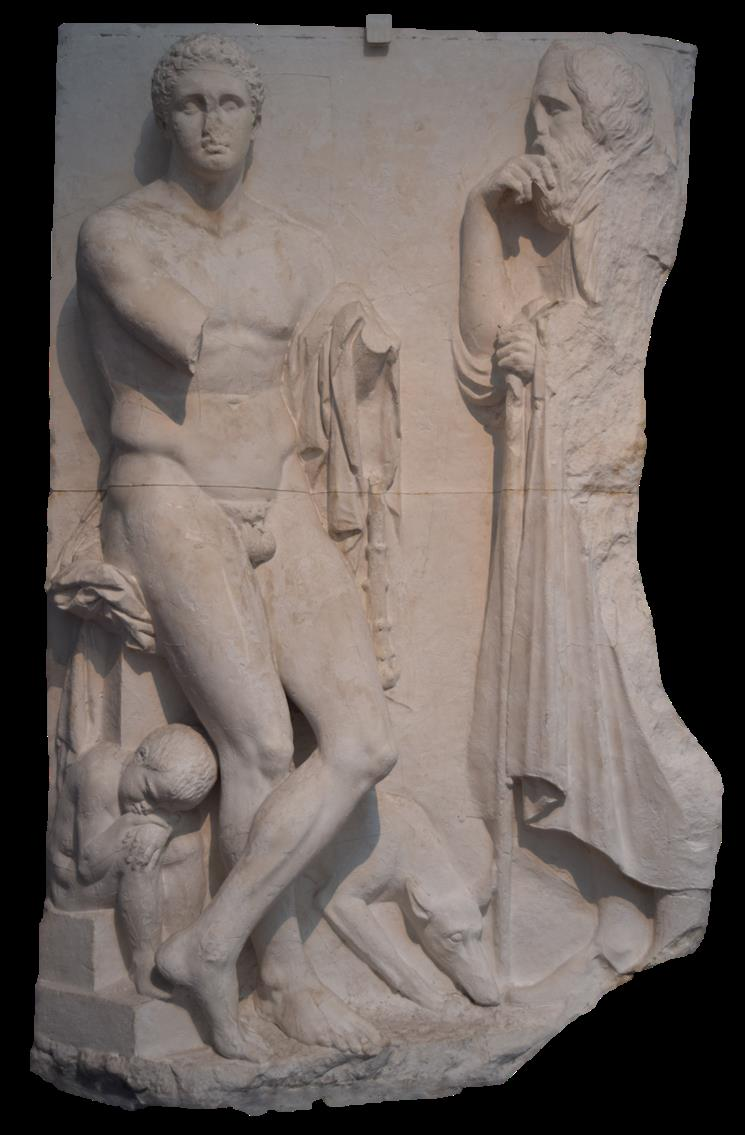
\includegraphics[width=.8\linewidth]{Robson_Figure_11}

	\caption{Ilissos relief. Oxford, Ashmolean Cast Gallery Inv. D076; Athens, National Archaeological Museum Inv. 869; 340-330 \BC, Pentelic Marble. Ilissos River, Athens (Found in 1874); Height: 1.68m, Width: 1.07m; Bibliography: TCG, 218, D076; CAT 2, 821-4, 2950; DAG 2, 226, 1055.211.
		Comparanda: NAM, inv. 731; inv. 871.
		{\normalfont\scriptsize \\ \copyright\ by Joseph Robson}}
	\label{fig:Robson_Figure_11}
\end{figure}
\clearpage
\begin{figure}[!p]
	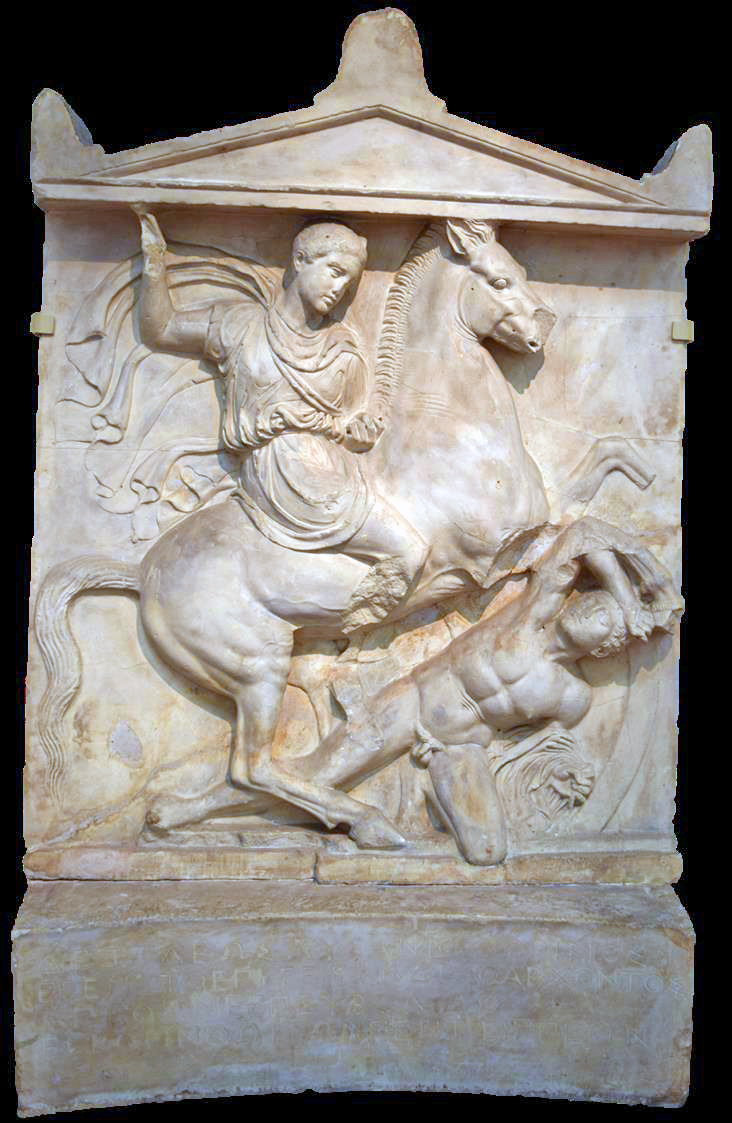
\includegraphics[width=.8\linewidth]{Robson_Figure_12}

	\caption{Grave stele of Dexileos. Oxford, Ashmolean Cast Gallery Inv. D067; Athens, Kerameikos Museum Inv. P1130; 394-393 \BC Pentelic Marble; Athenian Kerameikos (Found in 1863 in the family precinct of Dexileos); Height: 1.75m, Width: 1.35m; Bibliography: TCG, 216, D067; CAT 2, 143-5, 2.209; DAG 2, 254-5, 1158.248.
		Comparanda: D066; NAM, inv. 2744; inv. 3708; inv. 3620a.
		{\normalfont\scriptsize \\ \copyright\ by Joseph Robson}}
	\label{fig:Robson_Figure_12}
\end{figure}

\clearpage
\begin{figure}[!p]
	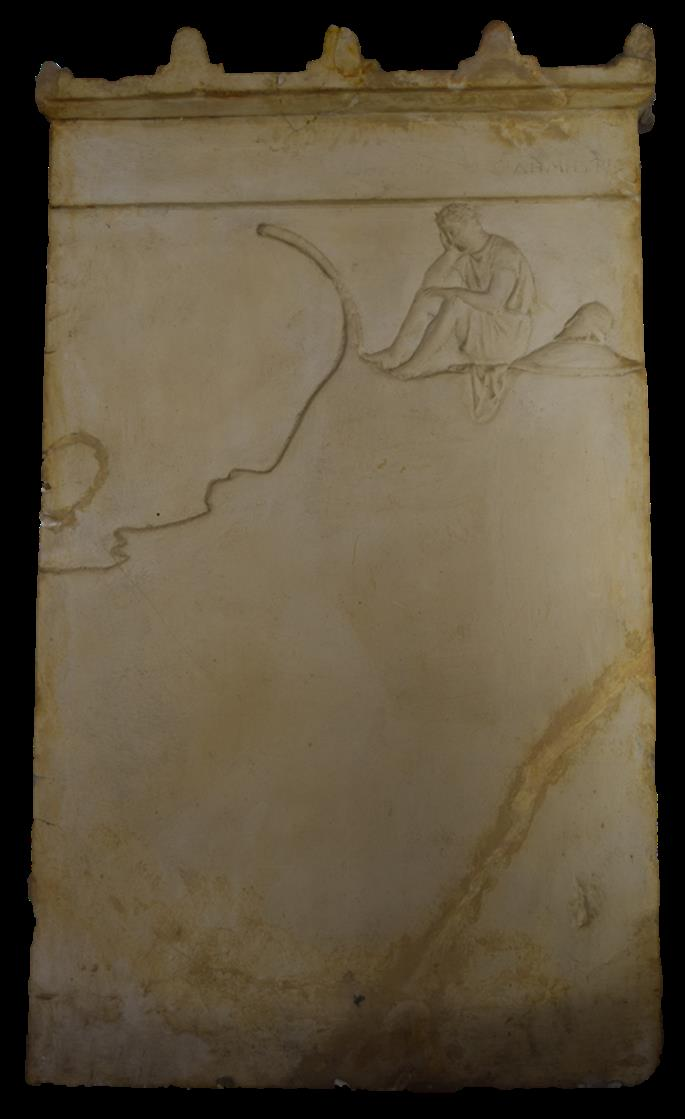
\includegraphics[width=.8\linewidth]{Robson_Figure_13}

	\caption{Grave stele of Demokleides. Oxford, Ashmolean Cast Gallery Inv. D064. Athens, National Archaeological Museum Inv. 752; 400-375 BC, Marble. Athens (Found in 1881); Height: 60cm, Width: 45cm; Bibliography: TCG, 215, D064; CAT 1, 316-7, 1.330; DAG 2, 623.122.
		{\normalfont\scriptsize\\ \copyright\ by Joseph Robson}}
	\label{fig:Robson_Figure_13}
\end{figure}
\clearpage
\begin{figure}[!p]
	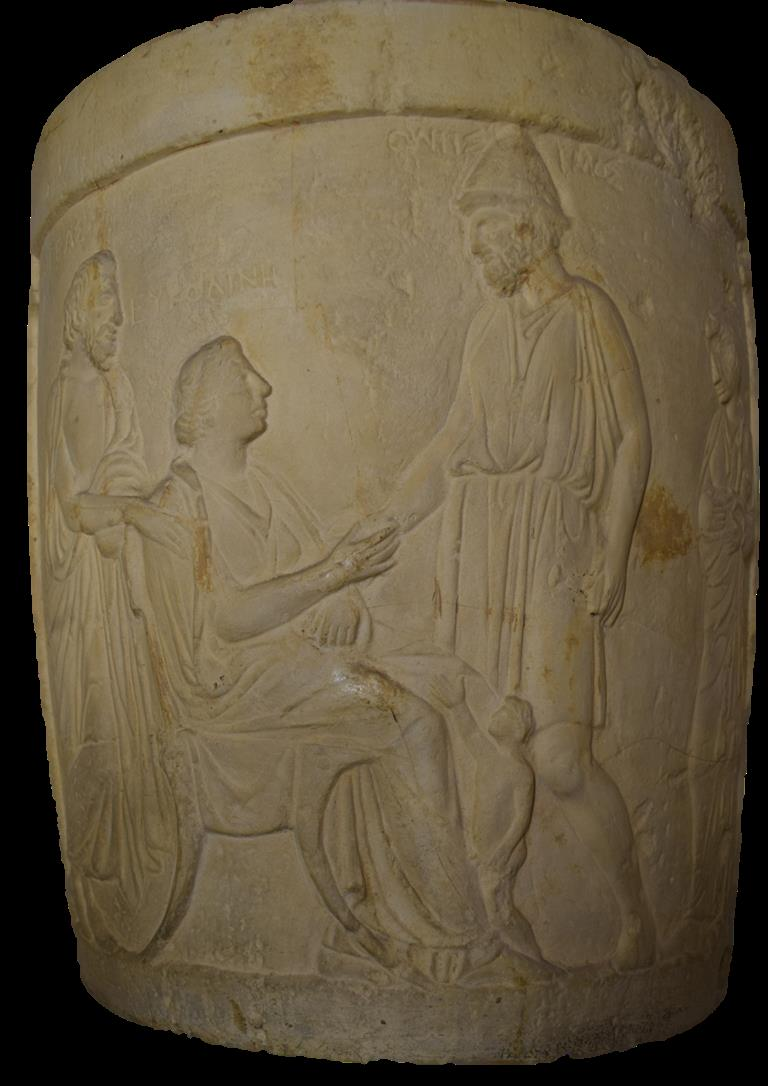
\includegraphics[width=\linewidth]{Robson_Figure_14}

	\caption{Funerary lekythos of Onesimos; Oxford, Ashmolean Cast Gallery Inv. D065; Munich, Glyptothek Inv. 209; C.405 BC, Pentelic Marble; Odos Aiolou, Athens (Found in 1811); Height: 48cm, Width: 45cm, Diameter: 20cm; Bibliography: TCG, 215, D065; DAG 1, 87-8, 380.92.
		Comparanda: D069; NAM, inv. 815.
		{\normalfont\scriptsize \\ \copyright\ by Joseph Robson}}
	\label{fig:Robson_Figure_14}
\end{figure}
\clearpage
\IJSRAclosing%<---- don't change this!
